% Fakesection 序言之前

\RequirePackage[l2tabu, orthodox]{nag}
\RequirePackage{ifxetex}
\RequireXeTeX

\documentclass{article}

%颜色
\usepackage{xcolor}

%长度
\usepackage{printlen}
\uselengthunit{mm}

%图形
\usepackage{pifont}
\usepackage{ean13isbn}
\usepackage{qrcode}
\usepackage{pdfpages}
\usepackage{overpic}
\usepackage{graphicx}
\graphicspath{{./src/}}
\usepackage{media9}
\usepackage{wallpaper}
\usepackage{wrapfig}

%表格
\usepackage{tabu}
\usepackage{longtable}
\usepackage{booktabs}
\usepackage{diagbox}
\usepackage{multicol}
\usepackage{multirow}
\usepackage{makecell}
\usepackage{fancybox}
\usepackage{colortbl}
\usepackage{tcolorbox}
\tcbuselibrary{skins}
\tcbuselibrary{breakable}
\tcbuselibrary{theorems}
\tcbuselibrary{listings}
\tcbuselibrary{xparse}
\tcbuselibrary{minted}% 用minted排版代码
\usepackage{fvextra}
\usepackage{csvsimple}
\usepackage{boxedminipage2e}

%公式
\usepackage{amsmath}
\usepackage{amsthm}
\usepackage{amsfonts}
\usepackage{amssymb}
\usepackage{amsbsy}
\usepackage{amsopn}
\usepackage{amstext}
\usepackage{mathrsfs}
\usepackage{bm}
\usepackage{textcomp}
\usepackage{latexsym}
\usepackage{exscale}
\usepackage{relsize}
%\usepackage{xymtex}
\usepackage{physics}
\usepackage{siunitx}
\usepackage{hologo}
\usepackage{cases}

%文字
\usepackage{csquotes}
\usepackage{microtype}
\usepackage[heading=true]{ctex}
\setCJKfamilyfont{zhsong}[AutoFakeBold = {2.17}]{SimSun}
\renewcommand*{\songti}{\CJKfamily{zhsong}}

%正文
\usepackage{fancyhdr}
\usepackage{geometry}
\usepackage{lastpage}
\usepackage{indentfirst}
\usepackage{setspace}
\renewcommand\arraystretch{1}

%非正文
\usepackage{makeidx}
\makeindex
\usepackage{epigraph}
\usepackage{varwidth}
\usepackage{exercise}
\usepackage{tasks}

%参考文献
\usepackage{morewrites}
\renewcommand{\thefootnote}{\fnsymbol{footnote}}
\usepackage[resetlabels]{multibib}

%标题
\usepackage{caption}
\usepackage{subcaption}
\newcounter{sub}

%其它
\usepackage{atbegshi}
\usepackage{lipsum}

\csname
endofdump
\endcsname

%代码
\usepackage{minted}

%链接%与beamer 冲突
\usepackage
[	colorlinks = true,
linkcolor = gray,
citecolor = gray,
backref=page
]{hyperref}

%枚举%与beamer 干涉
\usepackage{enumitem}
\setlist[enumerate, 2]
{	fullwidth,
	label = \arabic*.,
	font = \textup,
	itemindent=2em
}

%标题%与beamer 冲突
\usepackage{titlesec}
%\titleformat{\chapter}{\centering\Huge\bfseries}{实验\chinese{chapter}~}{0pt}{}
\titleformat{\section}{\centering\LARGE\bfseries}{\S\ifthenelse{\value{section}=0}{}{\thesection}~}{0pt}{}
%\titleformat{\subsection}{\Large}{\chinese{subsection}、~}{0pt}{}
%\titleformat{\subsubsection}{\large}{\arabic{subsubsection}.~}{0pt}{}

\begin{document}

% Fakesection 扉页

\begin{titlepage}
	\centering

	\includegraphics[width=.8\linewidth]{NJUST.ai}

	\vspace{20mm}

	\textbf{\songti\zihao{-0}电工电子综合实验(II)}

	\begin{flushright}
		\textbf{\songti\zihao{1}——多功能数字钟的设计与实现}
	\end{flushright}

	\vspace{20mm}

	\begin{spacing}{1}

		\centering
		\zihao{2}

		\begin{tabu}to.8\linewidth{@{}X[4,r]@{}X[c]@{}X[12,l]@{}}
			\makebox[4\ccwd][s]{院系}     & :&\underline{\makebox[12\ccwd][c]{\kaishu{电子工程与光电技术学院}}}\\
			\makebox[4\ccwd][s]{班号}     & :&\underline{\makebox[12\ccwd][c]{\kaishu{9171040G11}}}\\
			\makebox[4\ccwd][s]{姓名}     & :&\underline{\makebox[12\ccwd][c]{\kaishu{吴振宇}}}\\
			\makebox[4\ccwd][s]{学号}     & :&\underline{\makebox[12\ccwd][c]{\kaishu{916101630117}}}\\
			\makebox[4\ccwd][s]{桌(组)号} & :&\underline{\makebox[12\ccwd][c]{\kaishu{11}}}\\
			\makebox[4\ccwd][s]{指导教师} & :&\underline{\makebox[12\ccwd][c]{\kaishu{刘学敏}}}\\
			\makebox[4\ccwd][s]{实验日期} & :&\underline{\makebox[12\ccwd][c]{\kaishu{\today}}}\\
			\makebox[4\ccwd][s]{成绩}     & :&\underline{\makebox[12\ccwd][c]{}}
		\end{tabu}

		\vspace{0mm}%缩进

	\end{spacing}

	\vspace{0mm}%缩进

\end{titlepage}

%页眉页脚%与book冲突
\pagestyle{fancy}
\renewcommand{\headrulewidth}{0pt}
\lhead{\small{\leftmark}}
\chead{\small{\rightmark}}
\rhead{\small{第\thepage 页~共~\pageref{LastPage}~页}}
\lfoot{}
\cfoot{}
\rfoot{}

% Fakesection 目录

\pagenumbering{roman}

\tableofcontents
\listoffigures
\listoftables
\setcounter{section}{-1}

\pagenumbering{arabic}

\newpage

\section{实验简介}%
\label{sec:实验简介}

设计制作一个0分00秒$ \sim $9分59秒的多功能计时器,设计要求如下: \cite{electron}

\begin{enumerate}
	\item 设计一个脉冲发生电路,为计时器提供秒脉冲(\SI{1}{Hz}),为报时电路提供驱动蜂鸣器的高低脉冲信号(\SI{1}{kHz}、\SI{2}{kHz});
	\item 设计计时电路:完成0分00秒$ \sim $9分59秒的计时、译码、显示功能;
	\item 设计清零电路:具有开机自动清零功能,并且在任何时候,按动清零开关,可以对计时器进行手动清零;
	\item 设计校分电路:在任何时候,拨动校分开关,可进行快速校分;(校分隔秒)
	\item 设计报时电路:使数字计时器从9分53秒开始报时,每隔一秒发一声,共发三声低音,一声高音;即9分53秒、9分55秒、9分57秒发低音(频率\SI{1}{kHz}),9分59秒发高音(频率\SI{2}{kHz});
	\item 系统级联。将以上电路进行级联完成计时器的所有功能;
	\item 可以增加数字计时器附加功能:定时、动态显示等。
\end{enumerate}

\section{总体设计}%
\label{sec:总体设计}

数字计时器由计时电路、译码显示电路、脉冲发生电路、校分电路、清零电路和报时电路这几部分组成。其原理框图如图\ref{fig:总体设计}: \cite{circuit}

\begin{figure}[htpb]
	\centering
	\includegraphics[width=0.8\linewidth]{clock.pdf}
	\caption{总体设计}
	\label{fig:总体设计}
\end{figure}

\begin{figure}[htpb]
	\centering
	\includegraphics[width=0.8\linewidth]{bread.pdf}
	\caption{实物图}
	\label{fig:实物图}
\end{figure}

原理图中最左边的常开开关1用于校分,最右边的常开开关0用于清零,最左上方的双刀双掷开关是电源总开关。拨码开关S用于定时和暂停,当S打到最上面时正常计时,当S打到下方时开始定时,20秒后会数码管自动停止变化,同时信号指示灯会从正常的闪烁状态进入熄灭状态。当S打到空挡时立刻暂停。拨码开关D打到不同档位,动态选通的频率会发生变化。

面包板一共有4块,故将电路分为3层,留1层方便功能扩展。从上到下数,第一层为显示层,包含数码管和显示译码器,是动态显示电路中显示的一部分;第二层为计数层,包含计数部分和动态显示电路根据显示的结果选择的部分;第三层是功能层,从左至右分别是校分电路、脉冲发生电路、报时电路、清零电路。

因为元器件限制,实际作品有部分与原理图不符。比如滑动变阻器只找到2个,只找到2个常开开关没有找到拨码开关。所以用\SI{0}{\ohm}电阻的插上与拔下代替拨码开关的开与关。用接插件代替双刀双掷开关。

电路布线大体采取了与原理图相似的方案,但由于面包板布局限制有微小改动。

为了方便排查错误,在布线之初就考虑了导线的颜色。比如电源线选红色,地线选黑色,清零信号线选蓝色,时钟信号线选黄色,数据信号线选绿色,选通信号线选白色,芯片内部内部连线选无色。

\section{硬件设计}%
\label{sec:硬件设计}

\subsection{脉冲发生电路}%
\label{sub:脉冲发生电路}

振荡器是数字钟的核心。采用石英晶体构成振荡器电路,产生稳定的高频脉冲信号,作为数字钟的时间基准,再经过分频器输出标准秒脉冲(\SI{1}{Hz})。

分频器的功能主要有两个:

\begin{enumerate}
	\item 产生标准秒脉冲(\SI{1}{Hz});
	\item 提供功能扩展电路所需驱动脉冲信号(\SI{1}{kHz}、\SI{2}{kHz})。
\end{enumerate}

脉冲发生电路原理图如图\ref{fig:脉冲发生电路}所示:

\begin{figure}[htpb]
	\centering
	\includegraphics[
	width=0.6\linewidth,
	clip,
	trim=
	8.019cm
	2.1cm
	14.85cm
	12.6cm
	]{clock0.pdf}
	\caption{脉冲发生电路}
	\label{fig:脉冲发生电路}
\end{figure}

采用晶体的固有频率为$ 2^{15}\SI{}{Hz}= \SI{32768}{Hz} $。对$ 2^{15} $\SI{}{Hz}信号进行分频,得到\SI{1}{Hz}信号。分频器采用CD4060和74LS74来实现,CD4060如图\ref{fig:CD4060引脚图},为14位二进制串行计数器。CD4060内部有14级由T触发器构成的二分频器,但实际输出端只有10个:Q4$ \sim $Q10、Q12$ \sim $Q14。Q1$ \sim $Q3以及Q11并不引出。CP0为晶振电路的引出端,需接外部石英晶体。Cr为复零端,为高电平或正脉冲时振荡器停振。从输出功能看,CD4060能得到10种不同的分频系数,最小为$ 2^4 $分频,最大为$ 2^14 $分频,即将$ 2^15 $\SI{}{Hz}送入该芯片,最大分频输出Q14输出信号频率为\SI{2}{Hz}。

由于CD4060最多能完成14级二分频,所以还需要再加一级二分频,才能把4060输出的\SI{2}{Hz}信号变成秒信号。外接二分频器可采用D触发器(74LS74)构成的二分频电路,74LS74如图\ref{fig:74LS00引脚图},管脚功能如表\ref{tab:74LS74功能表}所示,该芯片有上片和下片两个D触发器,\SI{2}{Hz}信号经过二分频电路得到\SI{1}{Hz}的秒脉冲信号,即将D触发器的同相位输出Q端与触发信号D端连接在一起,复位端和控制端接电源,使该两端口无效,则Q端的输出信号即为\SI{1}{Hz}的秒脉冲信号。

\subsection{计时电路}%
\label{sub:计时电路}

计时电路如图\ref{fig:计时电路}所示,分位计数器和秒个位计数器均是从0$ \sim $9循环计数(模10计数),可采用CD4518或74LS161直接实现十进制计数功能;秒十位计数器为六进制计数器,需要将模10计数变换为一个从0$ \sim $5循环的模六计数。74LS21为四输入与门,片子内部封装两个相同且独立的四输入与门,该电路中只用到1个与门的2个输入,因此需要将该与门的其他两个输入端接\SI{5}{V}电源正极,不可悬空不接。

\begin{figure}[htpb]
	\centering
	\includegraphics[
	width=0.8\linewidth,
	clip,
	trim=
	2.97cm
	9.45cm
	16.632cm
	8.4cm
	]{clock0.pdf}
	\caption{计时电路}
	\label{fig:计时电路}
\end{figure}

搭建电路时,首先将所有芯片电源端(VCC和GND端)分别连接至\SI{5}{V}电源正、负极;对于秒个位计数器,将秒信号发生电路输出的秒信号(\SI{1}{Hz}信号)送入秒个位计数器的2CP端,同时2EN端接\SI{5}{V}电源+极,2Cr端接\SI{5}{V}电源-极(注意:当清零电路搭建完成后,需将清零电路的输出替换2Cr端的\SI{5}{V}电源-极),秒个位计数器即可完成$ 0\sim 9 $循环计数;对于秒十位计数器,将秒个位计数器的输出2QD端送入秒十位计数器的2EN端,完成秒个位到秒十位的进位(当秒个位计数器从9跳至0时,2QD端得到$ 0\sim 9 $循环计数过程中唯一的下降沿,将此下降沿送至秒十位计数器的2EN端,即可实现秒十位计数器加1,实现进位),同时2CP端接\SI{5}{V}电源+极,秒十位计数器即可在进位信号的驱动下完成$ 0\sim 5 $循环计数。对于分位计数器,将秒十位计数器的输出2QC端送入分位计数器的2EN端,完成秒十位到分位的进位(当秒十位计数器从5跳至0时,2QC端得到$ 0\sim 5 $循环计数过程中唯一的下降沿,将此下降沿送至分位计数器的2EN端,即可实现分位计数器加1,实现进位),同时2CP端接\SI{5}{V}电源+极,2Cr端接\SI{5}{V}电源负极(注意:当清零电路搭建完成后,需将清零电路的输出替换2Cr端的\SI{5}{V}电源-极),分位计数器即可完成$ 0\sim 9 $循环计数。

\subsection{译码显示电路}%
\label{sub:译码显示电路}

译码显示电路采用CD4511和2个数据选择器74LS157。作用是将计数器$ Q_A\sim Q_D $输出的二进制代码译成特定的输出信号以供显示器按代码的原意显示成数字,译码器采用CD4511七段字型译码器,由$ Q_A\sim Q_D $各脚输出段信号,以控制点亮LED数码管的字型段,CD4511的输入端ABCD依次接计数器的$ Q_A\sim Q_D $,即8421(BCD)码输出,CD4511有三个使能管脚,功能如表\ref{tab:CD4511功能表}所示。

\begin{figure}[htpb]
	\centering
	\includegraphics[
	width=0.8\linewidth,
	clip,
	trim=
	5.94cm
	9.45cm
	4.455cm
	1.05cm
	]{clock0.pdf}
	\caption{译码显示电路}
	\label{fig:译码显示电路}
\end{figure}

如图\ref{fig:7段数码管引脚图}和\ref{fig:7段数码管逻辑图},七段型发光二极管构成的数码显示器由高电压驱动,阴极共用,所以为共阴极。

电路从$ 0:00\sim 9:59 $循环计时,译码电路分别进行译码,采用共阴极七段LED数码管进行循环显示。CD4511的输入接到相应计数器的输出,而它的输出端与数码管的相应端相连,数码管通过\SI{300}{\ohm}的电阻接地,电路连接如图1.9所示。

\subsection{清零电路}%
\label{sub:清零电路}

\begin{wrapfigure}{r}{0.2\linewidth}
	\vspace{-10pt}
	\centering
	\includegraphics[
	width=\linewidth,
	clip,
	trim=
	23.166cm
	2.1cm
	4.455cm
	15.75cm
	]{clock0.pdf}
	\caption{清零电路}
	\label{fig:清零电路}
	\vspace{-10pt}
\end{wrapfigure}

该电路具有开机清零和手动清零功能。电路原理如图\ref{fig:清零电路}所示,将图\ref{fig:计时电路}计时电路的秒个位和分位的清零端即CD4518的管脚15(高电压有效)原来的接\SI{5}{V}电源-极导线拔开,将非门输出送至2Cr端,而秒十位CD4518的清零端原来接74LS21的输出,需要将此输出和图1.6中非门输出送入一个或门,再将或门输出送至秒十位CD4518的清零端,才能同时实现秒十位计数器的清零功能和模6计数功能。电路管脚连接如图1.7所示,对于清零电路,电路正常工作时开关打开,刚开机时,由于电容上的电压不能突变,电容两端初始为低电压,经过一个非门输出高电压,送到CD4518的2Cr端,整个计时电路清零,进而实现电路开机时清零,当电容充满电以后,非门的输入端为高电压,非门输出低电压,2Cr端无效,CD4518实现正常计数,电路正常工作。

按下开关后,电容、电阻组成一个回路,电容放电,当电容储存电量放完后,电容两端电压为低电压,即非门的输入端为低电压,非门输出高电压,送到CD4518的2Cr端,整个计时电路清零,进而实现电路手动清零。

\subsection{校分电路}%
\label{sub:校分电路}

当校分电路打到“正常”状态时,计数器正常计数;当开关打到“校分”状态时,秒个位和秒十位正常计数,分位进行快速校分,即分计数器可以不受秒计数器的进位信号的控制。校分电路的工作原理是:当校分开关在“1”电平,与非门2被选通,与非门1被封锁,秒进位产生的脉冲送至分计数器的时钟端;当开关打在“0”电平时,与非门1被选通,与非门2被封锁,校分信号送至分计数器的时钟端。

\begin{figure}[htpb]
	\centering
	\includegraphics[
	width=0.4\linewidth,
	clip,
	trim=
	2.97cm
	2.1cm
	22.275cm
	15.75cm
	]{clock0.pdf}
	\caption{校分电路}
	\label{fig:校分电路}
\end{figure}

\subsection{仿电台报时电路}%
\label{sub:仿电台报时电路}

用需要报时的时刻所对应的计数器的输出作为触发信号来驱动蜂鸣器报时,因为需要在9分53秒、9分55秒、9分57秒各报出一个低音,在9分59秒报出一个高音。具体设计过程如下:\cite{technology}

将各时刻各位对应的二进制码作如下图的比较:

\begin{enumerate}
	\item 通过卡诺图化简,将秒个位的3(0011)、5(0101)、7(0111)取或;
	\item 将1中所得结果和分位的9(1001)与再和秒十位的5(0101)与,所得的结果和\SI{1}{kHz}的信号与就可得到在9分53秒、9分55秒、9分57秒报出低音的驱动信号;
	\item 将分位的9(1001)和秒十位的5(0101)与再和秒个位的9(1001)与再和\SI{2}{kHz}的信号与就得到在9分59秒报出高音的驱动信号;
	\item 将2和3中得到的信号取或,就可以得到最终的报时驱动信号。
\end{enumerate}

\begin{figure}[htpb]
	\centering
	\includegraphics[
	width=0.6\linewidth,
	clip,
	trim=
	16.335cm
	2.1cm
	6.831cm
	15.75cm
	]{clock0.pdf}
	\caption{仿电台报时电路}
	\label{fig:仿电台报时电路}
\end{figure}

\section{功能测试}%
\label{sec:功能测试}

\begin{figure}[H]
	\centering
	\begin{subfigure}[htpb]{.45\linewidth}
		\centering
		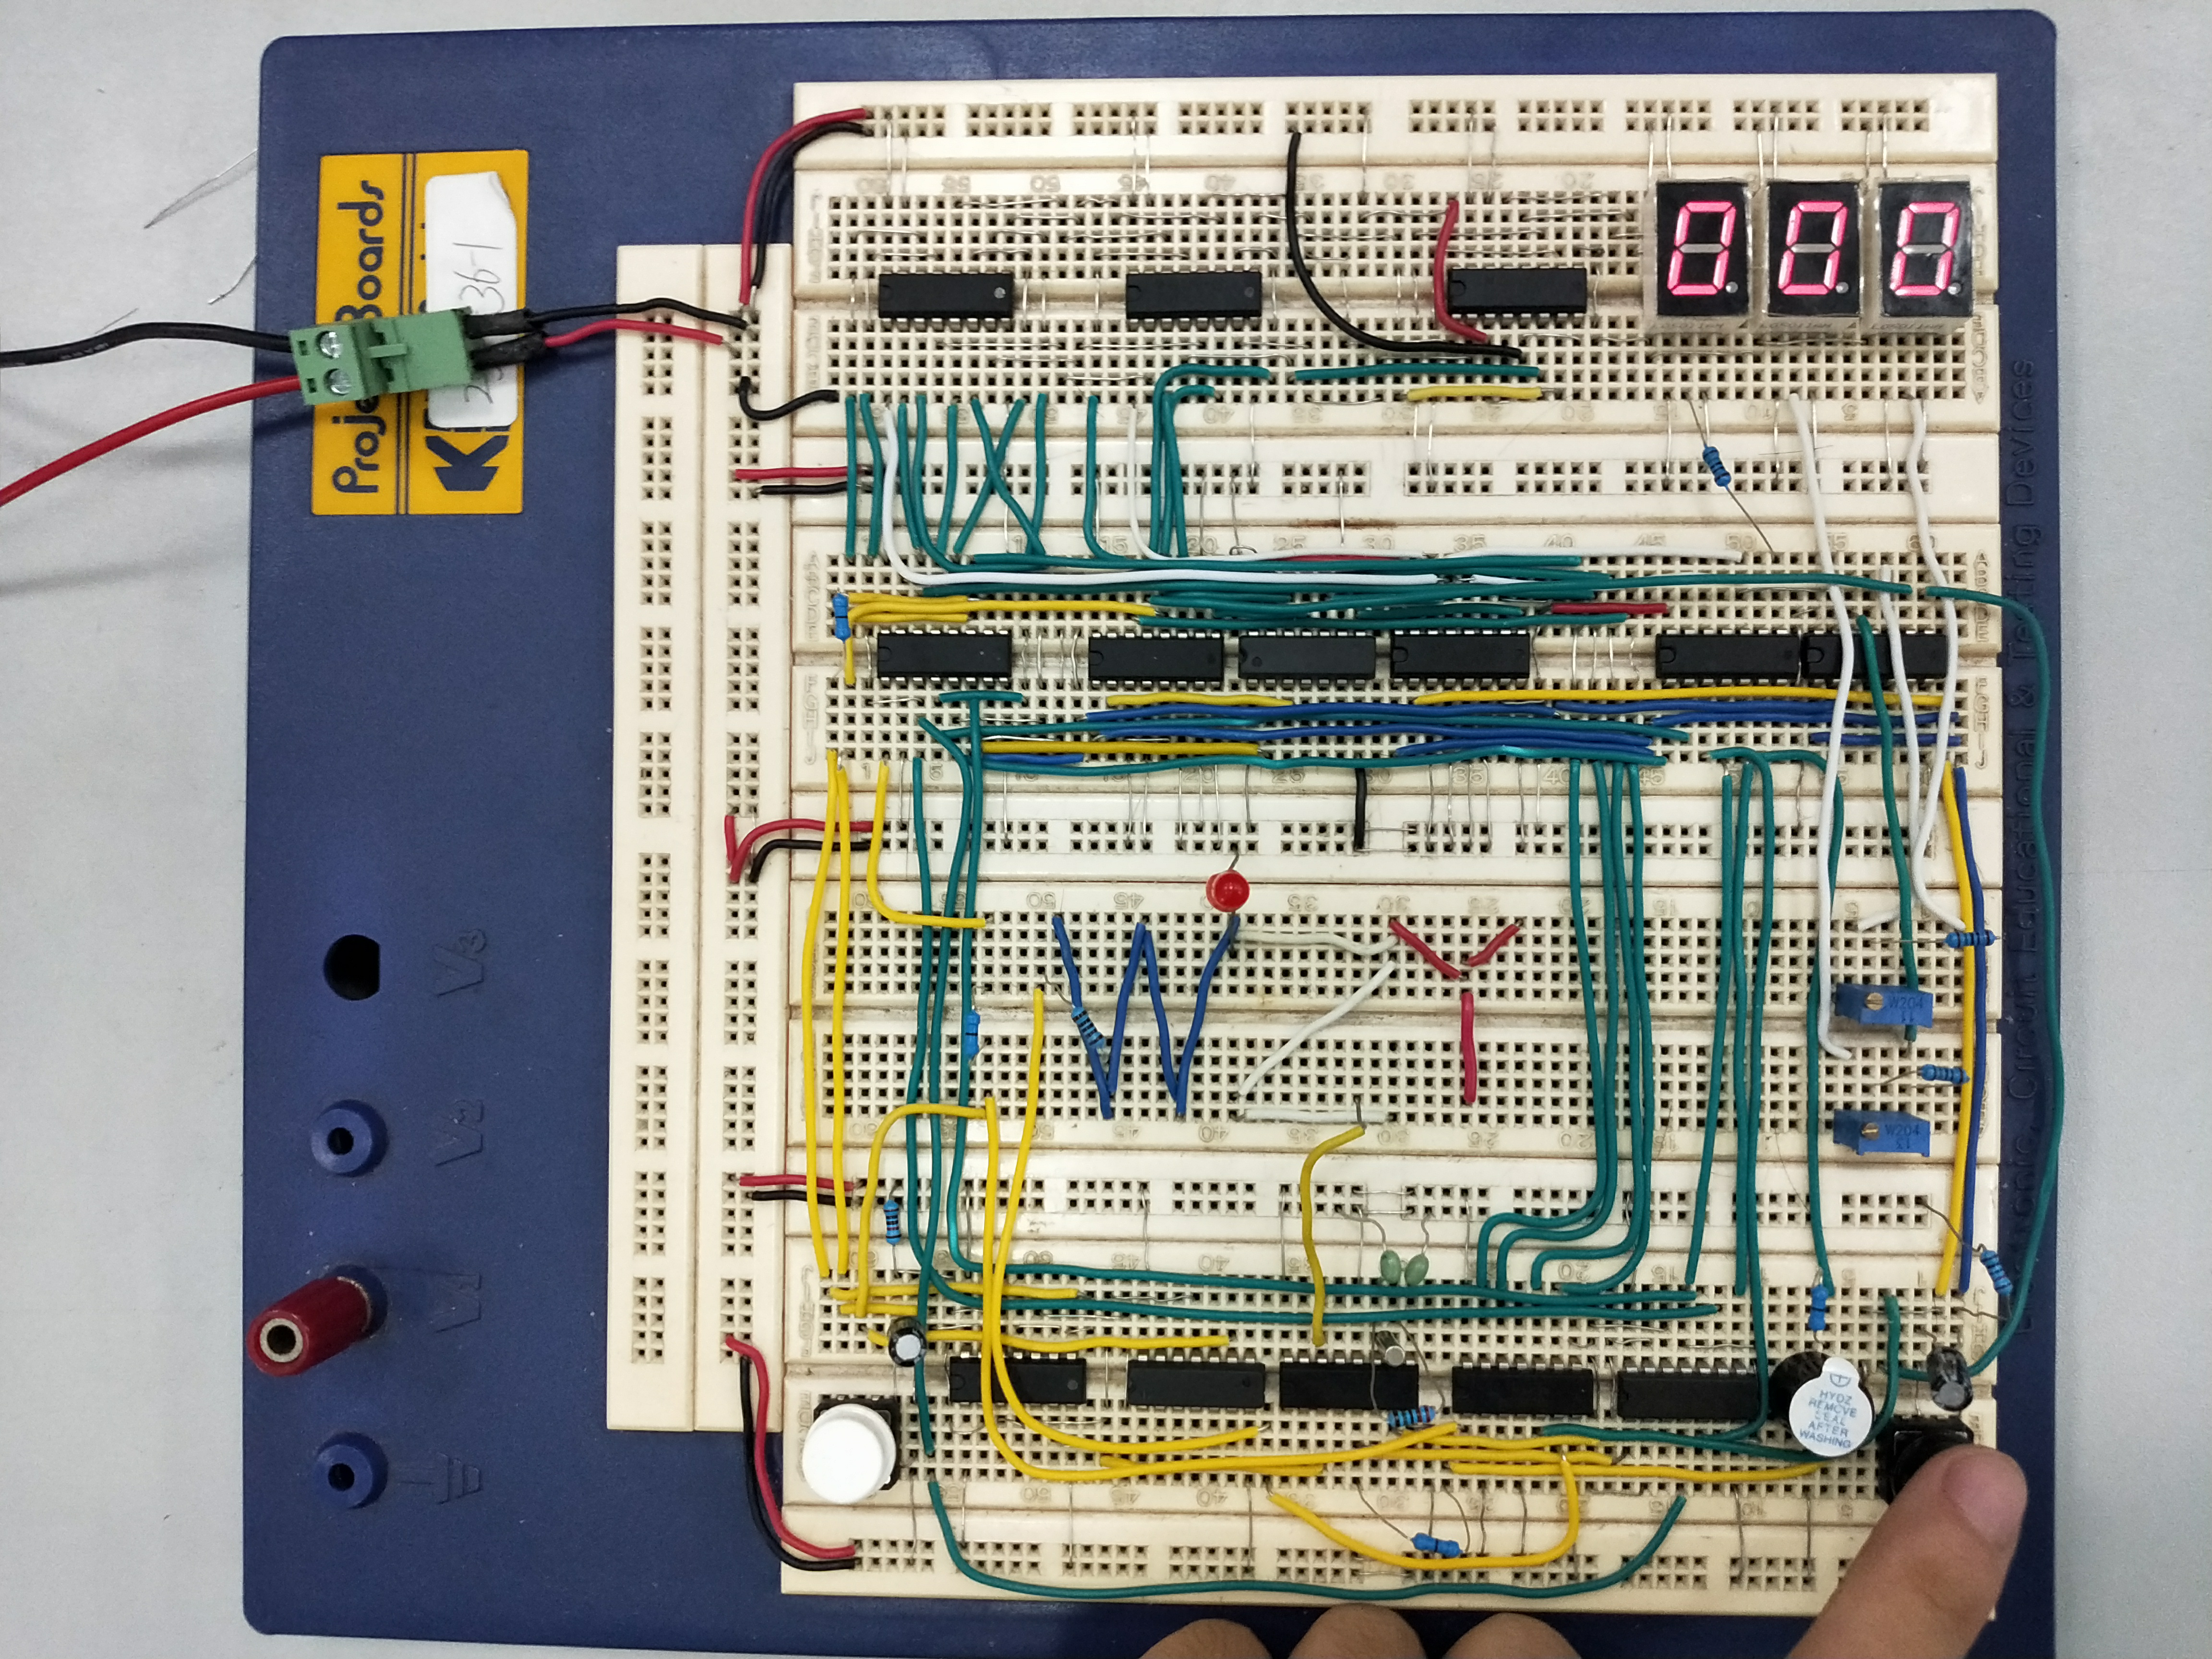
\includegraphics[width=\linewidth]{clear.png}
		\caption{清零}
		\label{fig:清零}
	\end{subfigure}
	\quad
	\begin{subfigure}[htpb]{.45\linewidth}
		\centering
		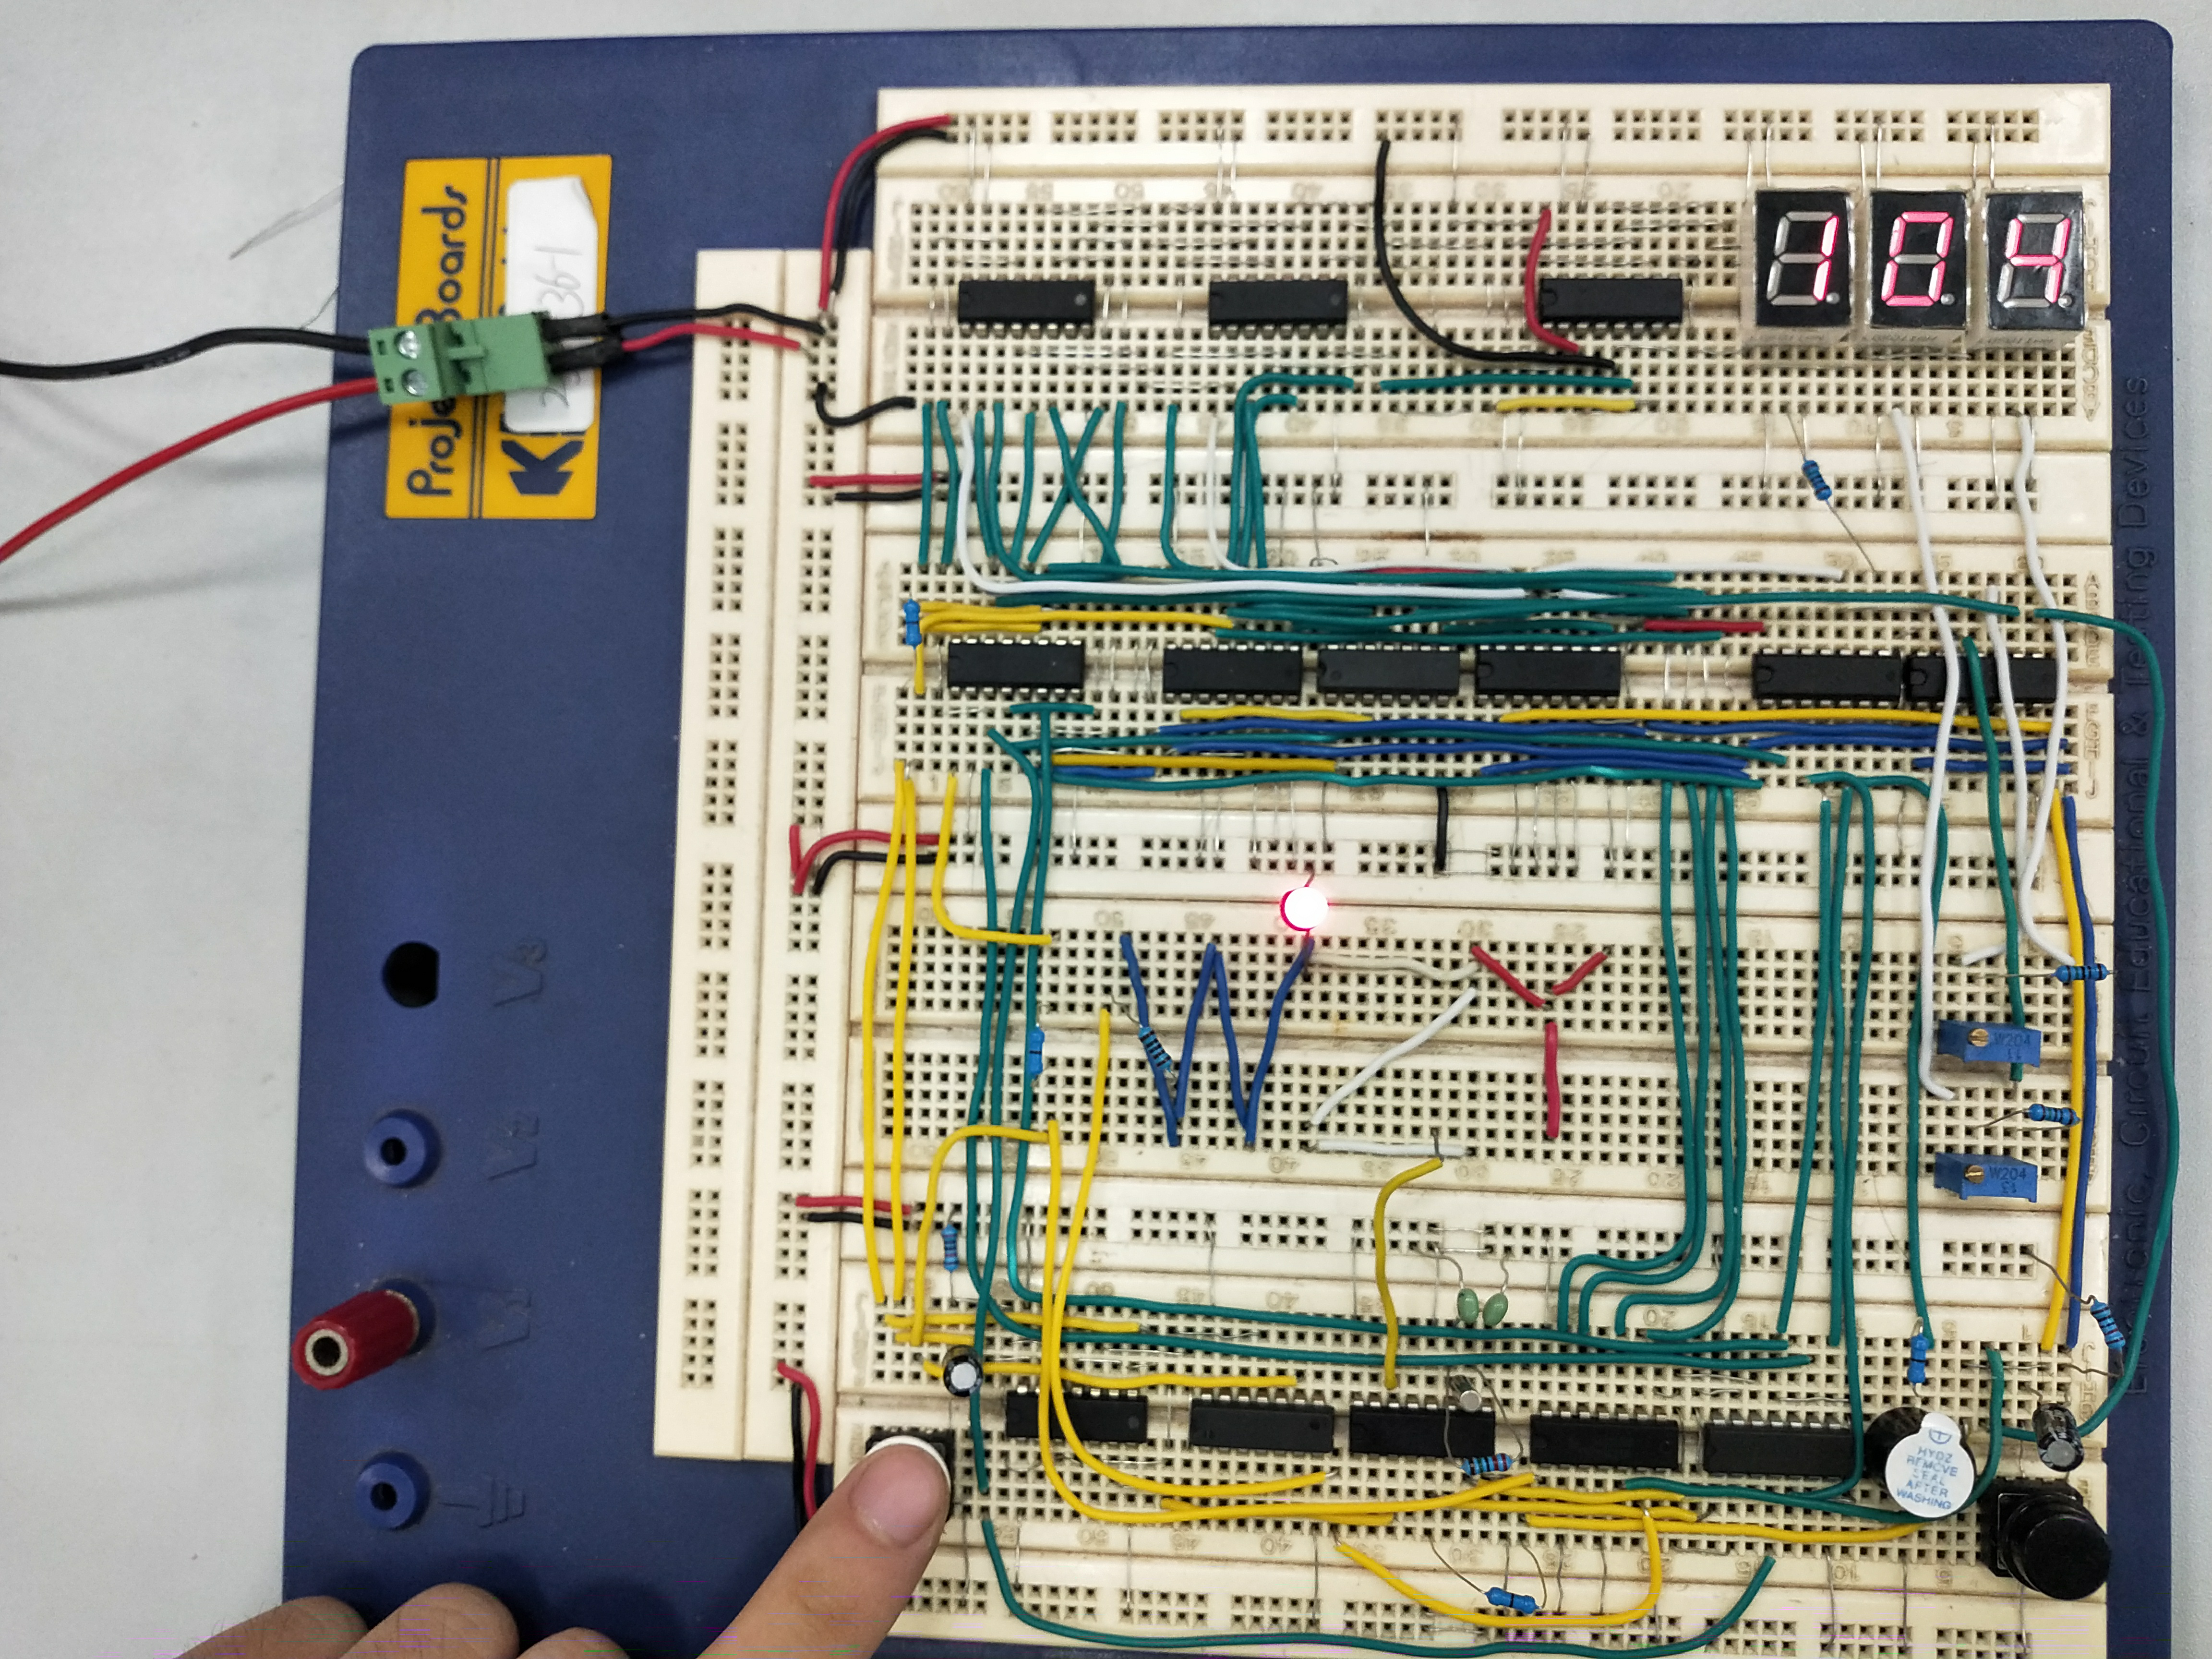
\includegraphics[width=\linewidth]{calibrate.png}
		\caption{校分}
		\label{fig:校分}
	\end{subfigure}
	\quad
	\begin{subfigure}[htpb]{.45\linewidth}
		\centering
		\includegraphics[width=\linewidth]{alarm.png}
		\caption{报时}
		\label{fig:报时}
	\end{subfigure}
	\quad
	\begin{subfigure}[htpb]{.45\linewidth}
		\centering
		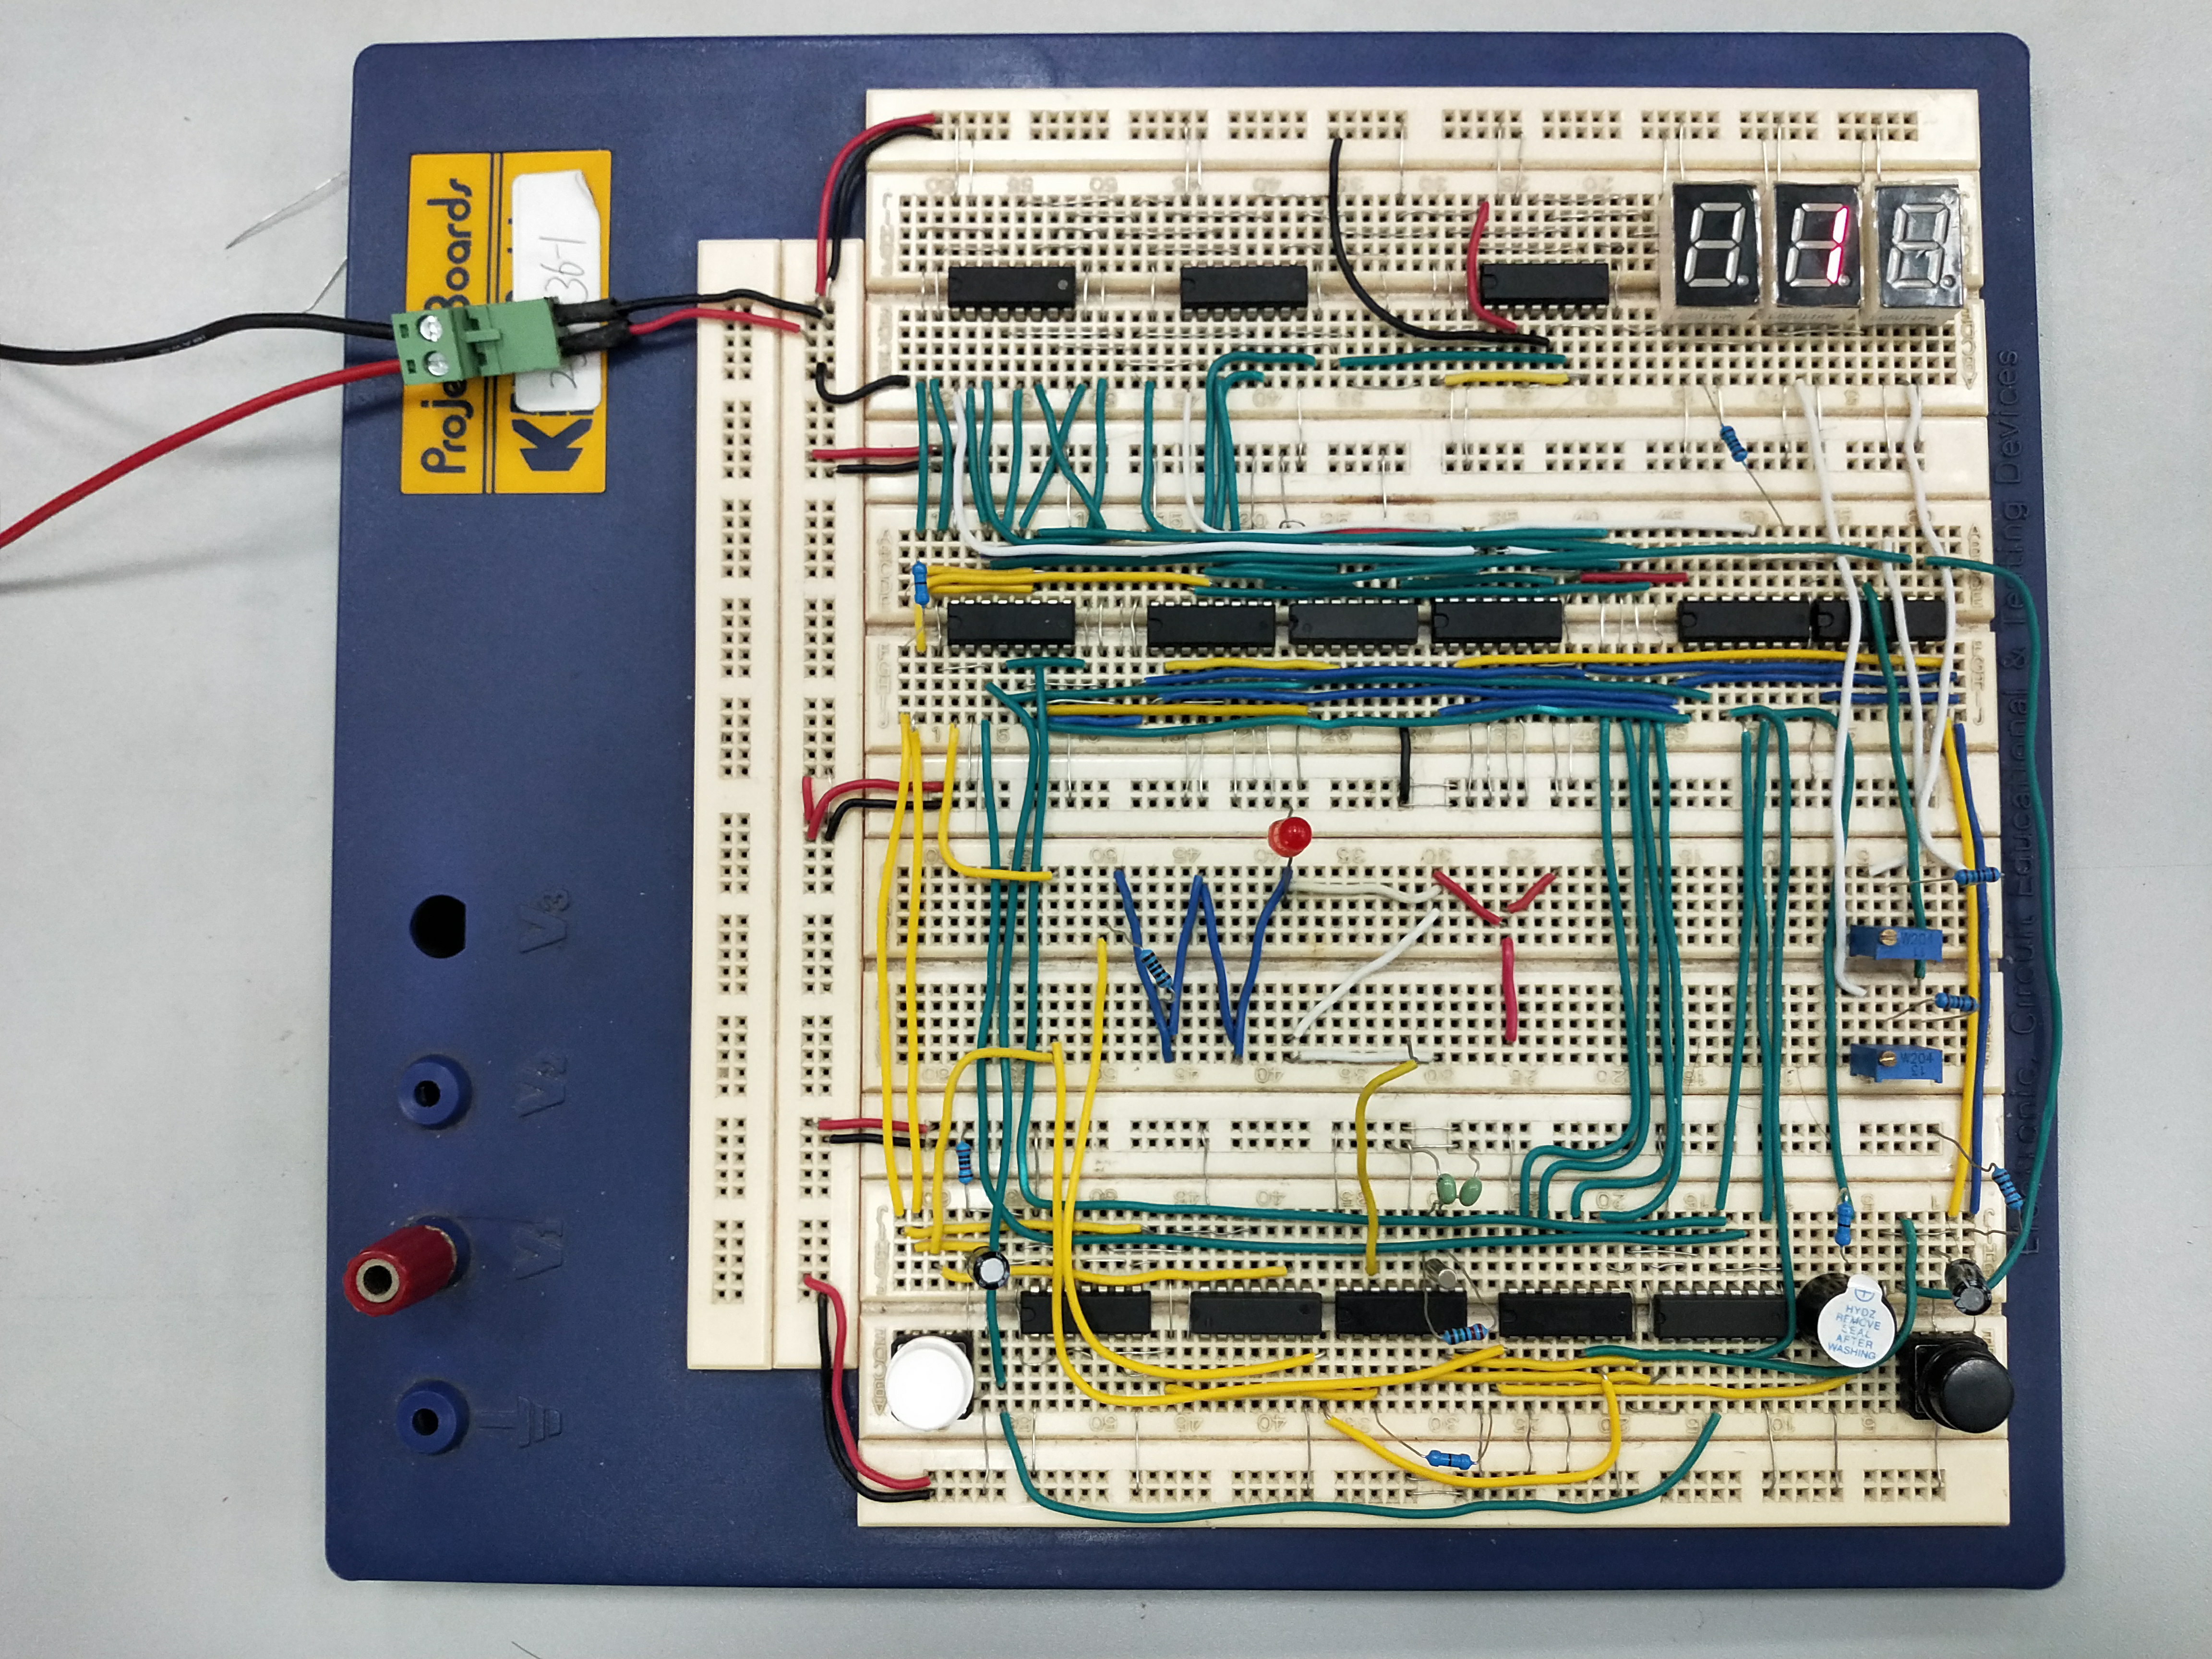
\includegraphics[width=\linewidth]{scan.png}
		\caption{动态显示频率改变}
		\label{fig:动态显示频率改变}
	\end{subfigure}
	\quad
	\begin{subfigure}[htpb]{.45\linewidth}
		\centering
		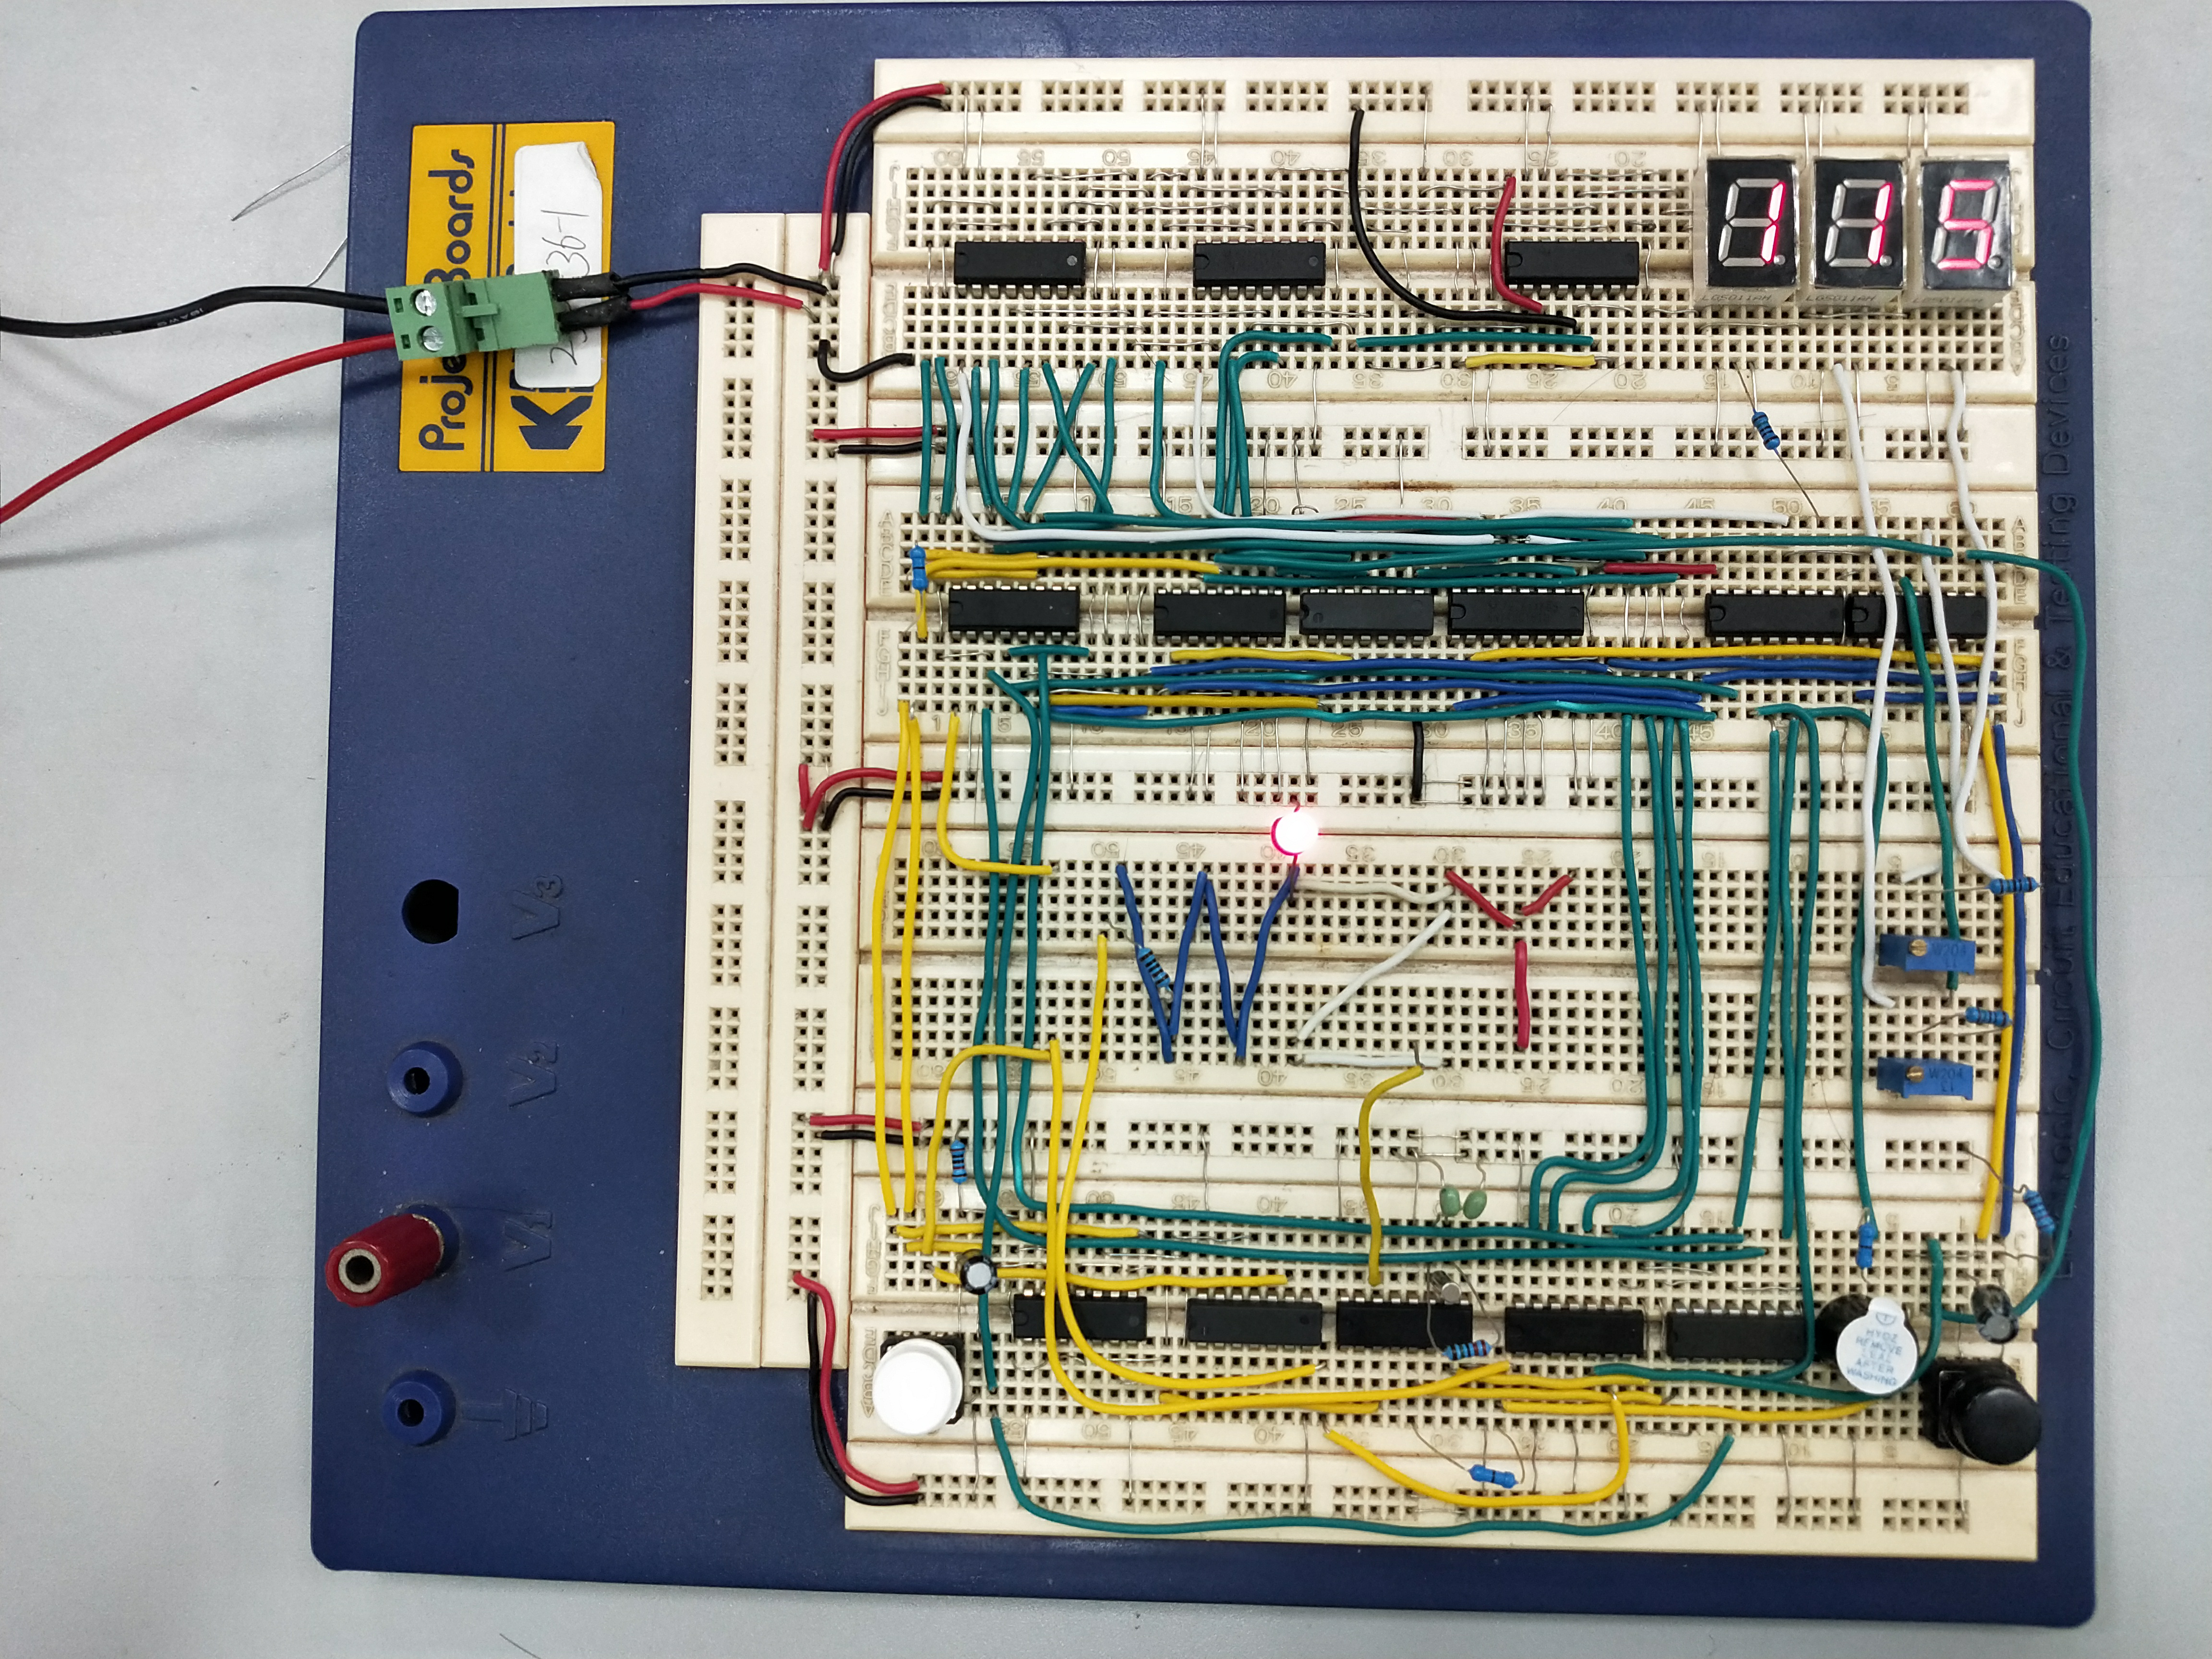
\includegraphics[width=\linewidth]{stop.png}
		\caption{暂停}
		\label{fig:暂停}
	\end{subfigure}
	\quad
	\begin{subfigure}[htpb]{.45\linewidth}
		\centering
		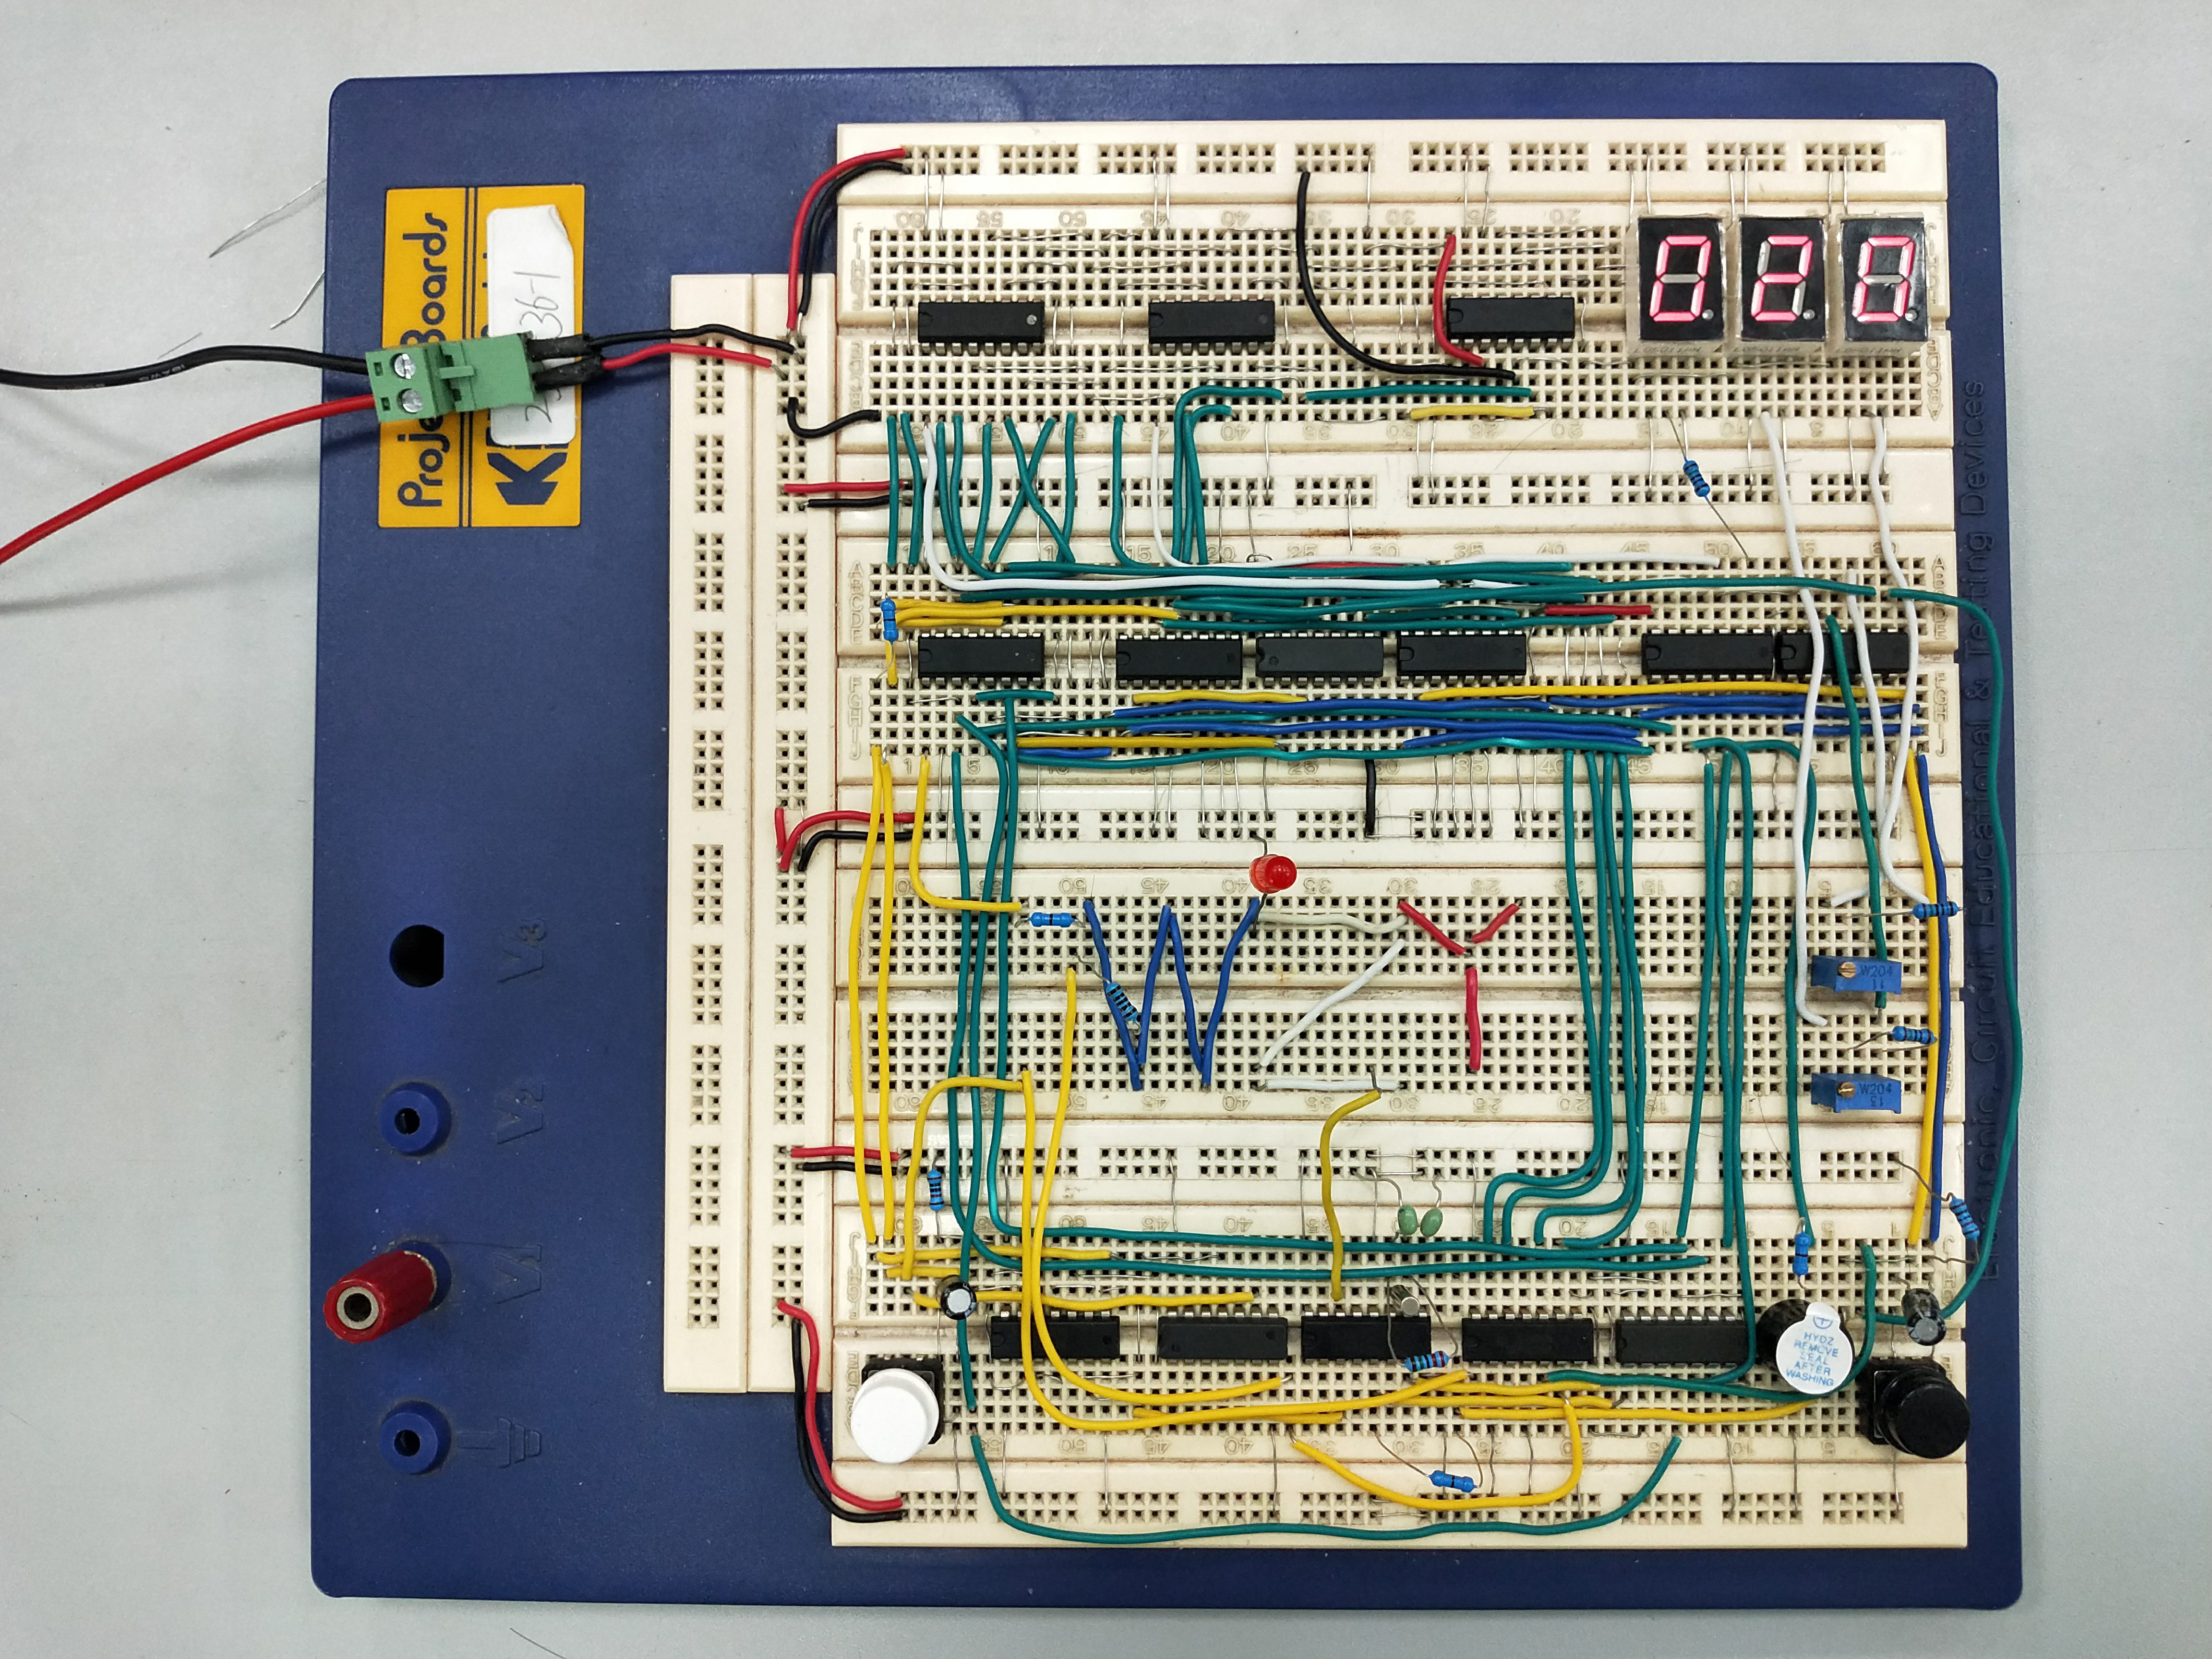
\includegraphics[width=\linewidth]{timer.png}
		\caption{定时}
		\label{fig:定时}
	\end{subfigure}
	\caption{功能测试}
	\label{fig:功能测试}
\end{figure}

\newpage

\section{实验感悟}%
\label{sec:实验感悟}

在仿真、布局和布线上花了较多的时间。因为布局较好的缘故,布线之后基本没有故障就能正常工作。个人感觉本作品是布局最清楚明了的。

\section{创新性分析}%
\label{sec:创新性分析}

\begin{enumerate}
	\item 完全平行布线,美观且更容易维护,元器件合理布局,例如3个数码管放在一起,方便查看时间;
	\item 在基础要求之上增加了动态显示、定时、暂停、动态显示频率改变、亮度调节等功能,并且有意预留了一部分用于以后功能扩展;
	\item 采用了接插件、开关等元器件,更加稳定和安全,方便操作;
	\item 尽可能的重复利用逻辑门芯片的门,减少元器件使用;
	\item 配套的仿真文件清楚明了,与实际布线相近,方便后续维护。
\end{enumerate}

\clearpage

% Fakesection 参考文献

\bibliographystyle{IEEEtran}
\bibliography{src/main}

\addcontentsline{toc}{section}{附录}

% Fakesection 附录

\appendix

\section{材料清单}%
\label{sec:材料清单}

\begin{table}[htpb]
	\centering
	\caption{元件清单}
	\label{tab:元件清单}
	\csvreader[
	head to column names,
	tabular=|c|c|c|,
	table head=\hline
	名称&型号&数量
	\\
	\hline,
	late after line=\\
	\hline
	]{src/bom.csv}{}{ \a&\b&\c }
\end{table}

\begin{table}[htpb]
	\centering
	\caption{工具清单}
	\label{tab:工具清单}
	\csvreader[
	head to column names,
	tabular=|c|c|c|,
	table head=\hline
	名称&型号&数量
	\\
	\hline,
	late after line=\\
	\hline
	]{src/tool.csv}{}{ \a&\b&\c }
\end{table}

\section{芯片手册}%
\label{sec:芯片手册}

\subsection{CD4060}%
\label{sub:CD4060}

\begin{figure}[H]
	\centering
	\includegraphics[width=0.6\linewidth]{CD4060.png}
	\caption{CD4060引脚图}
	\label{fig:CD4060引脚图}
\end{figure}

\newpage

\subsection{74LS74}%
\label{sub:74LS74}

\begin{figure}[H]
	\centering
	\includegraphics[width=0.6\linewidth]{74LS74.png}
	\caption{74LS74引脚图}
	\label{fig:74LS74引脚图}
\end{figure}

\begin{table}[H]
	\centering
	\caption{74LS74功能表}
	\begin{tabu}to.6\linewidth{@{}|X[c]|X[c]|X[c]|X[c]|X[c]|X[c]|@{}}
		\hline
		\multicolumn{4}{|c|}{输入} & \multicolumn{2}{c|}{输出} \\\hline
		PR & CLR &     CLK      & D &    Q    &  $ \overline{Q} $  \\ \hline
		0  &  1  &      X       & X &    1    &         0          \\ \hline
		1  &  0  &      X       & X &    0    &         1          \\ \hline
		0  &  0  &      X       & X &   1*    &         1*         \\ \hline
		1  &  1  & $ \uparrow $ & 1 &    1    &         0          \\ \hline
		1  &  1  & $ \uparrow $ & 0 &    0    &         1          \\ \hline
		1  &  1  &      0       & X & $ Q_0 $ & $ \overline{Q_0} $ \\ \hline
	\end{tabu}
	\label{tab:74LS74功能表}
\end{table}

\newpage

\subsection{74LS161}%
\label{sub:74LS161}

\begin{table}[H]
	\centering
	\caption{74LS161功能表}
	\begin{tabu}to\linewidth{@{}|X[2,c]|X[c]|X[c]|X[c]|X[c]|X[c]|X[c]|X[c]|X[c]|X[c]|X[c]|X[c]|X[c]|X[c]|X[2,c]|@{}}
		\hline
		& \multicolumn{9}{c|}{输入} & \multicolumn{5}{c|}{输出} \\\hline
		& CP & $ \overline{\mathrm{Cr}} $ & $ \overline{\mathrm{Cr}} $ & $ S_1 $ & $ S_0 $ & D & C & B & A & $ Q_D $ & $ Q_C $ & $ Q_B $ & $ Q_A $ & $ Q_{cc} $ \\\hline
		清零 & X & 0 & X & X & X & X & X & X & X & 0 & 0 & 0 & 0 & 0 \\\hline
		送数 & $ \uparrow $ & 1 & 0 & X & X & d & c & b & a & d & c & b & a & $ 0\rightarrow1 $ \\\hline
	\end{tabu}
	\label{tab:74LS161功能表}
\end{table}

\begin{figure}[H]
	\centering
	\includegraphics[width=.5\linewidth]{74LS161.png}
	\caption{74LS161引脚图}
	\label{fig:74LS161引脚图}
\end{figure}

\newpage

\subsection{CD4518}%
\label{sub:CD4518}

\begin{table}[H]
	\centering
	\caption{CD4518功能表}
	\begin{tabu}to.8\linewidth{@{}|X[2,c]|X[c]|X[c]|X[c]|X[c]|X[c]|X[c]|X[c]|@{}}
		\hline
		& \multicolumn{3}{c|}{输入} & \multicolumn{4}{c|}{输出} \\\hline
		& Cr & CP & EN & $ Q_D $ & $ Q_C $ & $ Q_B $ & $ Q_A $ \\\hline
		清零 & 1 & X & X & 0 & 0 & 0 & 0 \\\hline
		计数 & 0 & $ \uparrow $ & 1 & \multicolumn{4}{c|}{BCD码加法计数} \\\hline
		保持 & 0 & X & 0 & \multicolumn{4}{c|}{保持} \\\hline
		计数 & 0 & 0 & $ \downarrow $ & \multicolumn{4}{c|}{BCD码加法计数} \\\hline
		保持 & 0 & 1 & X & \multicolumn{4}{c|}{保持} \\\hline
	\end{tabu}
	\label{tab:CD4518功能表}
\end{table}

\begin{figure}[H]
	\centering
	\includegraphics[width=.5\linewidth]{CD4518.png}
	\caption{CD4518引脚图}
	\label{fig:CD4518引脚图}
\end{figure}

\newpage

\subsection{7段数码管}%
\label{sub:7段数码管}

\begin{figure}[H]
	\centering
	\includegraphics[width=.2\linewidth]{7seg.png}
	\caption{7段数码管引脚图}
	\label{fig:7段数码管引脚图}
\end{figure}

\begin{figure}[H]
	\centering
	\includegraphics[width=0.8\linewidth]{7seg-logic.png}
	\caption{7段数码管逻辑图}
	\label{fig:7段数码管逻辑图}
\end{figure}

\newpage

\subsection{CD4511}%
\label{sub:CD4511}

\begin{table}[H]
	\centering
	\caption{CD4511功能表}
	\begin{tabu}to\linewidth{@{}|X[2,c]|X[c]|X[c]|X[c]|X[c]|X[c]|X[c]|X[c]|X[c]|X[c]|X[c]|X[c]|X[c]|X[c]|X[c]|X[2,c]|@{}}
		\hline
		& \multicolumn{7}{c|}{输入} & \multicolumn{8}{c|}{字符} \\\hline
		& $ \overline{LT} $ & $ \overline{BI} $ & LE & D & C & B & A & g & f & e & d & c & b & a & 字符 \\\hline
		测灯 & 0 & X & X & X & X & X & X & 1 & 1 & 1 & 1 & 1 & 1 & 1 & 8 \\\hline
		灭零 & 1 & 0 & X & 0 & 0 & 0 & 0 & 0 & 0 & 0 & 0 & 0 & 0 & 0 & 消隐 \\\hline
		锁存 & 1 & 1 & 1 & X & X & X & X & \multicolumn{8}{c|}{显示$ LE=0\rightarrow 1 $时数据} \\\hline
			 & 1 & 1 & 0 & 0 & 0 & 0 & 0 & 0 & 1 & 1 & 1 & 1 & 1 & 1 & 0 \\\hline
			 & 1 & 1 & 0 & 0 & 0 & 0 & 1 & 0 & 0 & 0 & 1 & 1 & 1 & 0 & 1 \\\hline
			 & 1 & 1 & 0 & 0 & 0 & 1 & 0 & 1 & 0 & 1 & 0 & 0 & 1 & 1 & 2 \\\hline
			 & 1 & 1 & 0 & 0 & 0 & 1 & 1 & 1 & 0 & 0 & 1 & 1 & 1 & 1 & 3 \\\hline
			 & 1 & 1 & 0 & 0 & 1 & 0 & 0 & 1 & 1 & 0 & 1 & 1 & 1 & 0 & 4 \\\hline
			 & 1 & 1 & 0 & 0 & 1 & 0 & 1 & 1 & 1 & 0 & 1 & 1 & 0 & 1 & 5 \\\hline
			 & 1 & 1 & 0 & 0 & 1 & 1 & 0 & 1 & 1 & 1 & 1 & 1 & 0 & 0 & 6 \\\hline
			 & 1 & 1 & 0 & 0 & 1 & 1 & 1 & 0 & 0 & 0 & 1 & 1 & 1 & 1 & 7 \\\hline
			 & 1 & 1 & 0 & 1 & 0 & 0 & 0 & 1 & 1 & 1 & 1 & 1 & 1 & 1 & 8 \\\hline
			 & 1 & 1 & 0 & 1 & 0 & 0 & 1 & 1 & 1 & 0 & 1 & 1 & 1 & 1 & 9 \\\hline
	\end{tabu}
	\label{tab:CD4511功能表}
\end{table}

\begin{figure}[H]
	\centering
	\includegraphics[width=.5\linewidth]{CD4511.png}
	\caption{CD4511引脚图}
	\label{fig:CD4511引脚图}
\end{figure}

\newpage

\subsection{74LS00}%
\label{sub:74LS00}

\begin{table}[H]
	\centering
	\caption{74LS00功能表}
	\label{tab:74LS00功能表}
	\begin{tabu}to.3\linewidth{@{}|X[c]|X[c]|X[c]|@{}}
		\hline
		A & B & Y \\\hline
		0 & 0 & 1 \\\hline
		0 & 1 & 1 \\\hline
		1 & 0 & 1 \\\hline
		1 & 1 & 0 \\\hline
	\end{tabu}
\end{table}

\begin{figure}[H]
	\centering
	\includegraphics[width=.5\linewidth]{74LS00.png}
	\caption{74LS00引脚图}
	\label{fig:74LS00引脚图}
\end{figure}

\newpage

\subsection{74LS21}%
\label{sub:74LS21}

\begin{table}[H]
	\centering
	\caption{74LS21功能表}
	\label{tab:74LS21功能表}
	\begin{tabu}to.5\linewidth{@{}|X[c]|X[c]|X[c]|X[c]|X[c]|@{}}
		\hline
		A & B & C & D & Y \\\hline
		1 & 1 & 1 & 1 & 1 \\\hline
		0 & X & X & X & 0 \\\hline
		X & 0 & X & X & 0 \\\hline
		X & X & 0 & X & 0 \\\hline
		X & X & X & 0 & 0 \\\hline
	\end{tabu}
\end{table}

\begin{figure}[H]
	\centering
	\includegraphics[width=.5\linewidth]{74LS21.png}
	\caption{74LS21引脚图}
	\label{fig:74LS21引脚图}
\end{figure}

\newpage

\subsection{CD4069}%
\label{sub:CD4069}

\begin{table}[H]
	\centering
	\caption{CD4069功能表}
	\begin{tabu}to.2\linewidth{@{}|X[c]|X[c]|@{}}
		\hline
		A & $ \overline{A} $ \\\hline
		0 & 1 \\\hline
		1 & 0 \\\hline
	\end{tabu}
	\label{tab:CD4069功能表}
\end{table}

\begin{figure}[H]
	\centering
	\includegraphics[width=.5\linewidth]{CD4069.png}
	\caption{CD4069引脚图}
	\label{fig:CD4069引脚图}
\end{figure}

\newpage

\subsection{74LS32}%
\label{sub:74LS32}

\begin{table}[H]
	\centering
	\caption{74LS32功能表}
	\label{tab:74LS32功能表}
	\begin{tabu}to.3\linewidth{@{}|X[c]|X[c]|X[c]|@{}}
		\hline
		A & B & Y \\\hline
		0 & 0 & 0 \\\hline
		0 & 1 & 1 \\\hline
		1 & 0 & 1 \\\hline
		1 & 1 & 1 \\\hline
	\end{tabu}
\end{table}

\begin{figure}[H]
	\centering
	\includegraphics[width=.5\linewidth]{74LS32.png}
	\caption{74LS32引脚图}
	\label{fig:74LS32引脚图}
\end{figure}

\newpage

\subsection{74LS157}%
\label{sub:74LS157}

\begin{table}[H]
	\centering
	\caption{74LS157功能表}
	\begin{tabu}to.5\linewidth{@{}|X[c]|X[c]|X[c]|X[c]|X[c]|@{}}
		\hline
		\multicolumn{4}{|c|}{输入} & 输出 \\\hline
		G & S & A & B & Y \\\hline
		1 & X & X & X & 0 \\\hline
		0 & 0 & 0 & X & 0 \\\hline
		0 & 0 & 1 & X & 1 \\\hline
		0 & 1 & X & 0 & 0 \\\hline
		0 & 1 & X & 1 & 1 \\\hline
	\end{tabu}
	\label{tab:74LS157功能表}
\end{table}

\begin{figure}[H]
	\centering
	\includegraphics[width=.5\linewidth]{74LS157.png}
	\caption{74LS157引脚图}
	\label{fig:74LS157引脚图}
\end{figure}

\end{document}

